% Created 2023-11-17 vie 23:26
% Intended LaTeX compiler: pdflatex
\documentclass[11pt]{article}
\usepackage[utf8]{inputenc}
\usepackage[T1]{fontenc}
\usepackage{graphicx}
\usepackage{longtable}
\usepackage{wrapfig}
\usepackage{rotating}
\usepackage[normalem]{ulem}
\usepackage{amsmath}
\usepackage{amssymb}
\usepackage{capt-of}
\usepackage{hyperref}
\usepackage{../modern}
\bibliography{./fuentes.bib}
\raggedbottom
\setcounter{secnumdepth}{3}
\author{Luis Eduardo Galindo Amaya (1274895)}
\date{viernes, 17 noviembre 2023}
\title{Proyecto}
\hypersetup{
 pdfauthor={Luis Eduardo Galindo Amaya (1274895)},
 pdftitle={Proyecto},
 pdfkeywords={},
 pdfsubject={},
 pdfcreator={Emacs 28.1 (Org mode 9.5.2)}, 
 pdflang={Spanish}}
\begin{document}

\modentitlepage{../images/escudo-uabc-2022-color-cont.png}
\datasection{Individual}
\tableofcontents
\pagebreak

\section{Apoyo para programadores}
\label{sec:org75559d5}
\subsection{Aseguramiento de calidad de software}
\label{sec:org75d9a82}
Ayudar a los desarrolladores a identificar y corregir problemas en el
código antes de que se integre en el repositorio principal o antes de
realizar una implementación mediante técnicas de clean code. \\

Utilizar un analizador como Sonarlint permite enseñar buenas
técnicas de programación sin interferir con el desarrollo del proyecto,
se necesitaría invertir tiempo de capacitación en clean code además de
supervisión constante para evitar problemas de calidad en la rama
principal de trabajo.

\begin{figure}[htbp]
\centering
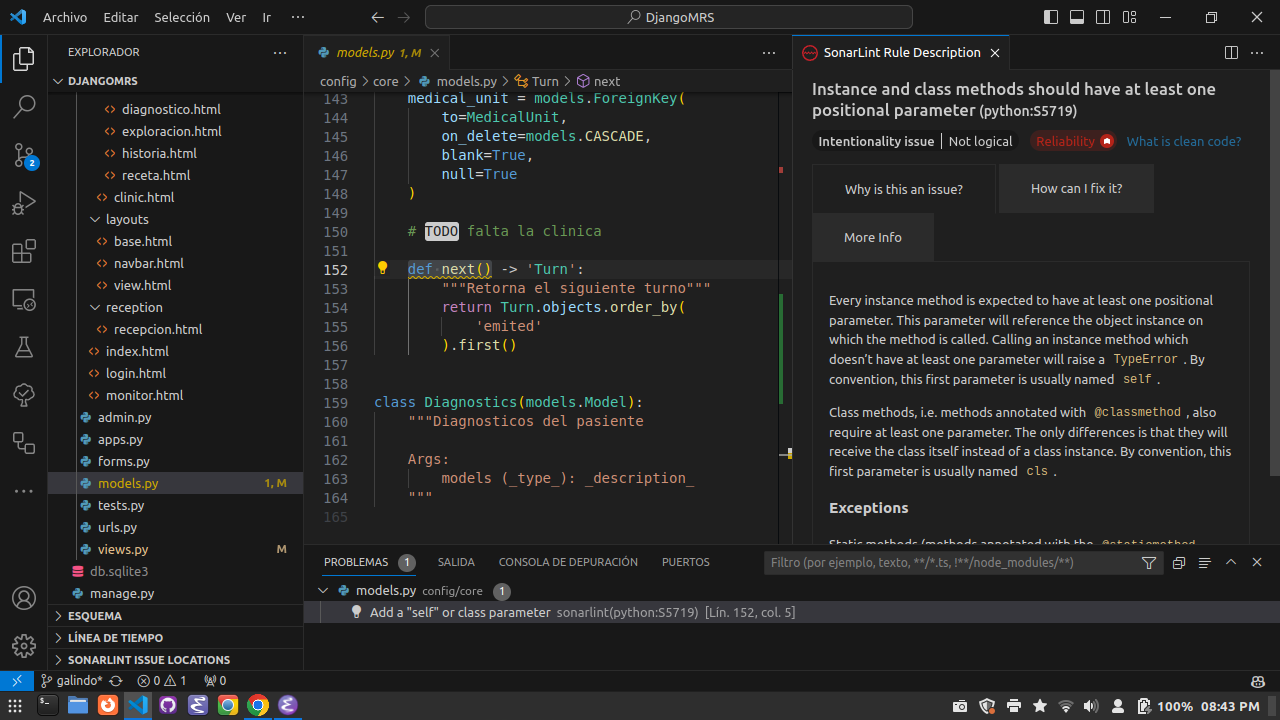
\includegraphics[width=10cm]{img/Captura de pantalla de 2023-11-17 20-43-45.png}
\caption{Plugin de Sonarlint}
\end{figure}

\begin{description}
\item[{Sonarlint}] \url{https://www.sonarsource.com/solutions/our-unique-approach/}
\end{description}

\pagebreak

\subsection{Generación de código}
\label{sec:orgde0634f}
GitHub Copilot es una herramienta desarrollada por GitHub en
colaboración con OpenAI que utiliza inteligencia artificial para
generar sugerencias de código mientras escribes. \\

Copilot permite a un desarrollador codificar de manera más ágil, esto
reduciendo la cantidad de tiempo que se pasa analizando la
documentación y nombrando cosas. Copilot en el futuro podría
reemplazar a algunos miembros del equipo, pero en el presente es una
herramienta de autocompletado muy útil ya que busca patrones comunes
en el código para hacer sus recomendaciones.  

\begin{figure}[htbp]
\centering
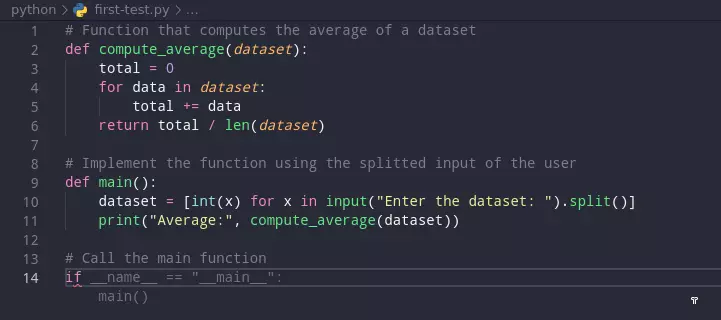
\includegraphics[width=10cm]{img/copilot.png}
\caption{Copilot recomendando código.}
\end{figure}

\subsection{Generación de pruebas unitarias}
\label{sec:orgf540ca0}
Las pruebas unitarias son una parte fundamental para el desarrollo de
aplicaciones modernas ya que nos permite verificar si el código cumple
con los requerimientos solicitados, la inteligencia artificial se
puede considerar en estos casos ya que, al no requerir de lógica,
solo requiere crear los casos de prueba. \\

Hacer pruebas unitarias requiere el tiempo del equipo además de
conocimientos de unit testing, utilizar IA podría permitir a equipos
menos experimentados utilizar el unit testing para mejorar la calidad
de sus productos de software.

\begin{figure}[htbp]
\centering
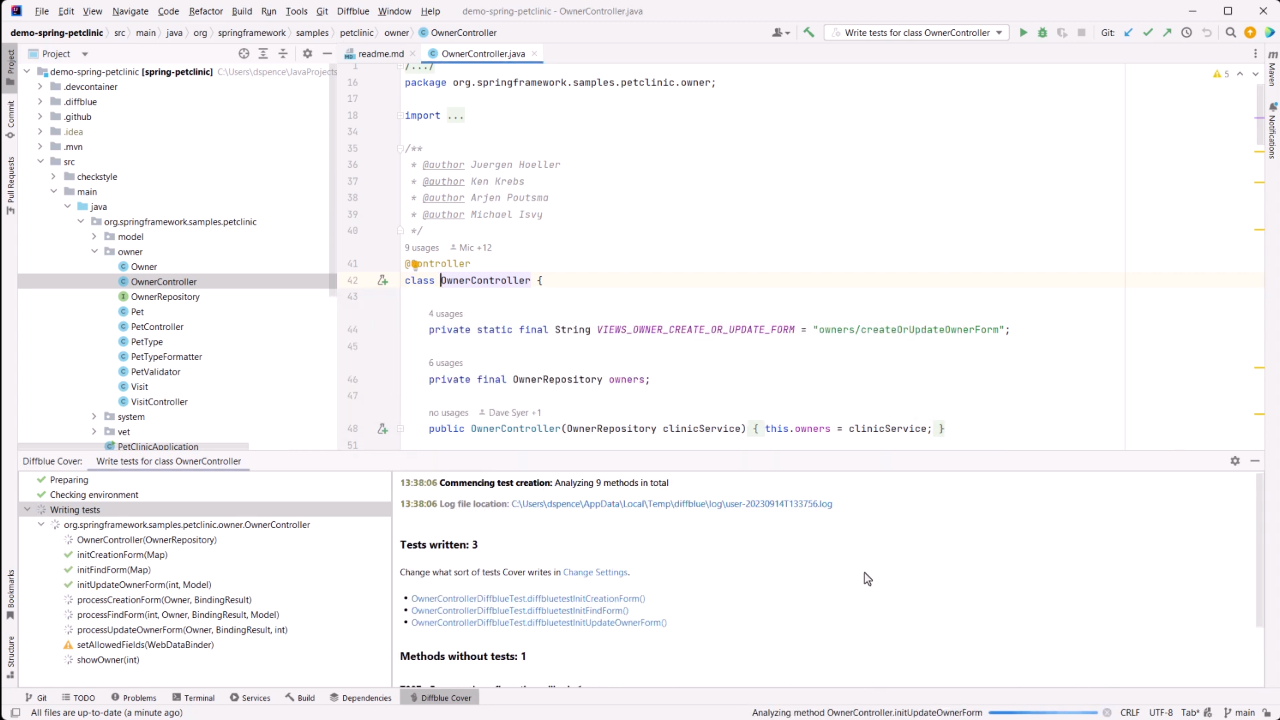
\includegraphics[width=8cm]{img/diffblue.png}
\caption{Diffblue generando pruebas unitarias en el panel inferior}
\end{figure}

\begin{description}
\item[{Diffblue}] \url{https://www.diffblue.com/}
\end{description}

\pagebreak

\section{Apoyo para diseñadores}
\label{sec:org5de3642}
\subsection{Análisis de diseño}
\label{sec:org97aba37}
Autify es una herramienta de inteligencia artificial que permite a los
diseñadores crear pruebas de uso en aplicaciones en múltiples
plataformas, probar si el contenido del correo electrónico es válido
para confirmar acciones. Acuerdo a los creadores de Autify el tiempo
de pruebas de usuarios es lo más tardado del desarrollo, Autify puede
reducir el número de personas requeridas para asegurar la
accesibilidad del mismo.  

\begin{figure}[htbp]
\centering
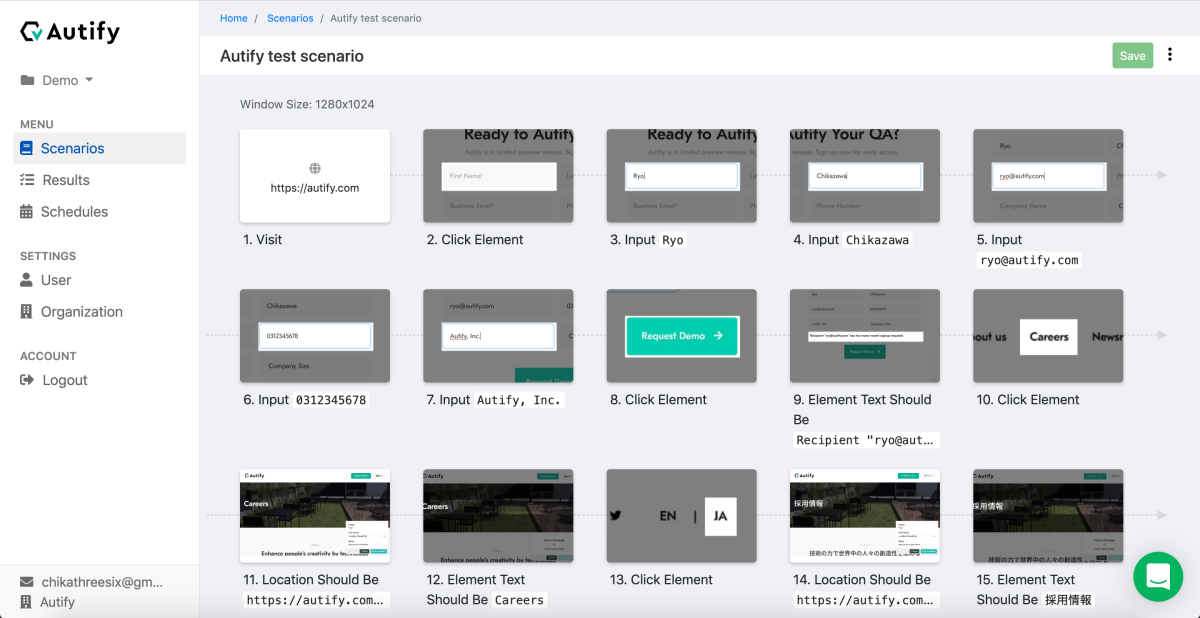
\includegraphics[width=9cm]{img/auty.png}
\caption{Resultados de Autify}
\end{figure}

\begin{description}
\item[{Autify}] \url{https://autify.com/}
\end{description}

\subsection{Generación de interfaces y prototipado}
\label{sec:org162a40d}
Framer permite a los diseñadores crear diseños de interfaz de usuario
avanzados con animaciones complejas, transiciones y comportamientos
interactivos. Esto es esencial para diseñar experiencias de usuario
atractivas y efectivas. Framer utiliza IA para generar prototipos
rápidos de páginas web, un prototipo rápido de una página permite a
los desarrolladores centrarse únicamente en la implementación de la
funcionalidad de esta. 

\begin{figure}[htbp]
\centering
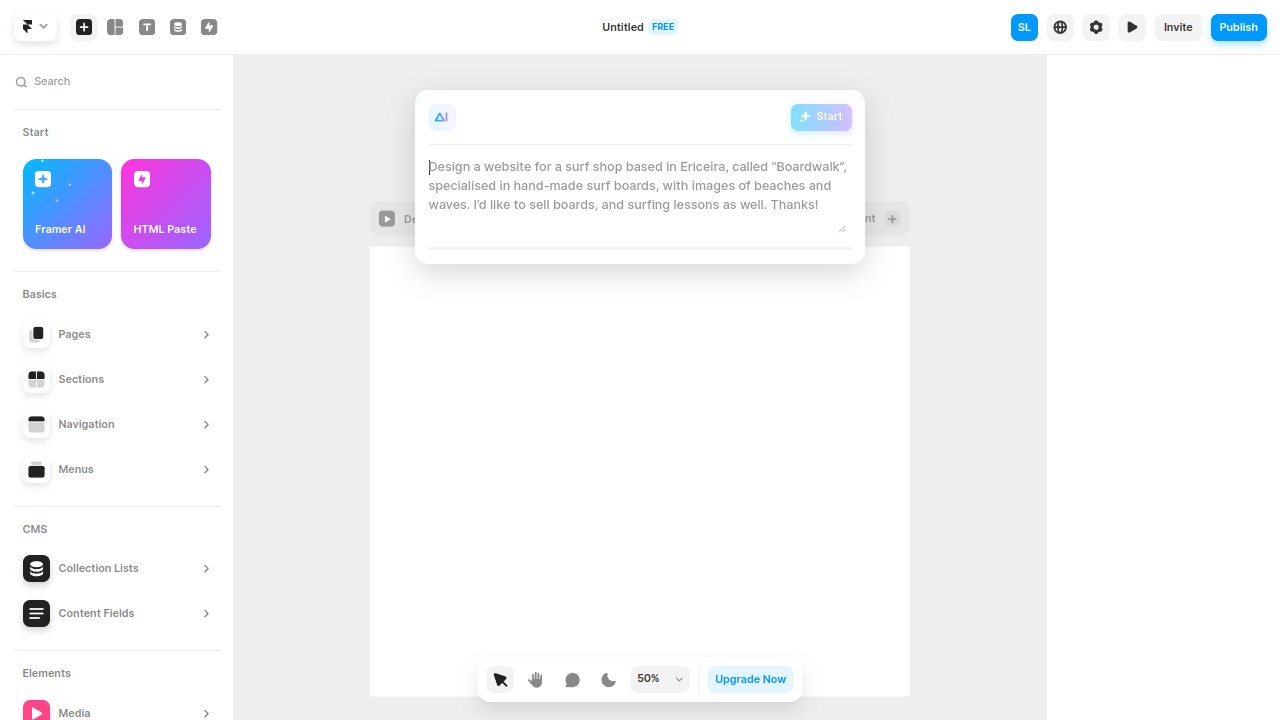
\includegraphics[width=10cm]{img/framer.png}
\caption{Framer pidiendo un prompt para generar el sitio.}
\end{figure}

\begin{description}
\item[{Framer}] \url{https://framer.com/}
\end{description}

\subsection{Generación de paletas de colores}
\label{sec:org1a16c40}
Huemint es una herramienta en línea que utiliza inteligencia
artificial (IA) para generar paletas de colores únicas, se basa en el
aprendizaje automático para determinar una paleta que se vea bien y
que no interfiera con la usabilidad. \\

Para elegir los colores se requeriría un equipo de diseñadores que
tengan conocimientos de UI.

\begin{figure}[htbp]
\centering
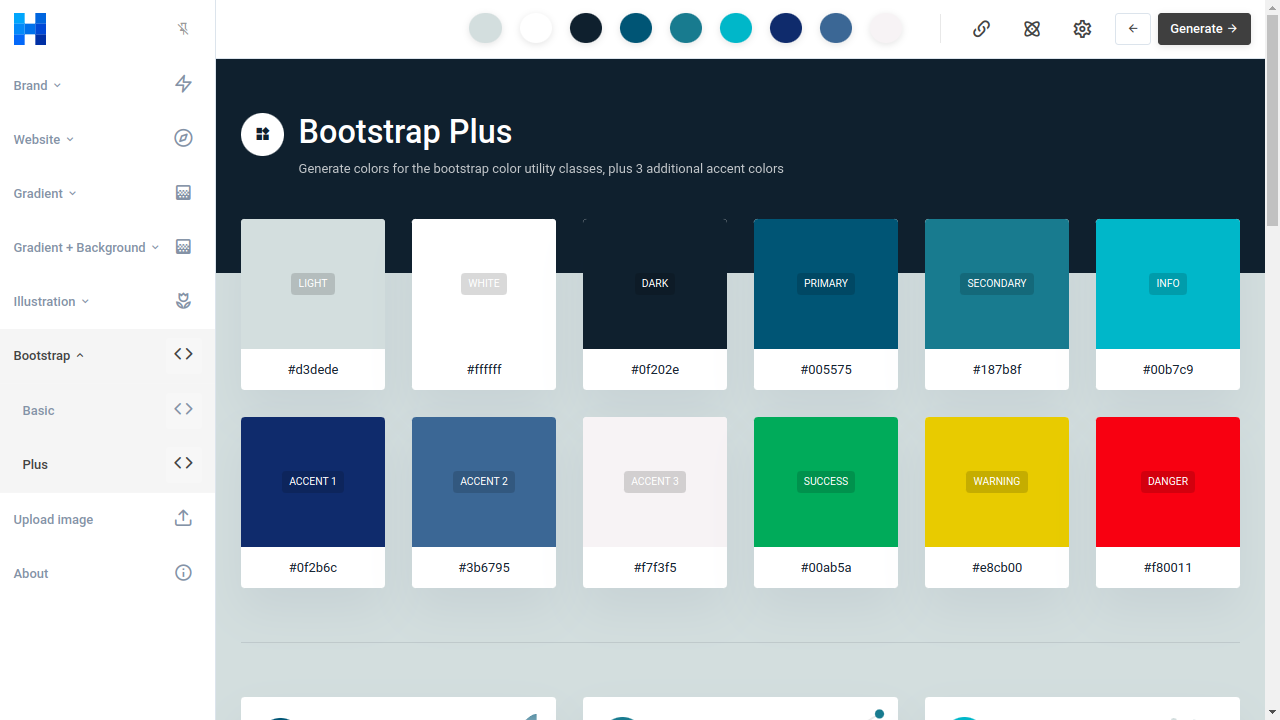
\includegraphics[width=10cm]{img/Huemint.png}
\caption{Huemint generando una paleta de colores}
\end{figure}

\begin{description}
\item[{Huemint}] \url{https://huemint.com/bootstrap-plus/}
\item[{Picular}] \url{https://picular.co/haskell\%20programing\%20lenguage}
\end{description}

\pagebreak

\section{Apoyo para el manejo de equipos}
\label{sec:org153beb9}
\subsection{Gestión de calendarios}
\label{sec:orgf297b1a}
Motion es una herramienta que permite gestionar calendarios y
planificar acciones a futuro, utiliza inteligencia artificial para
ajustar las tareas de manera más sencilla. \\

Reajustar los calendarios es una tarea que requiere de constante
supervisión y no puede descuidarse, herramientas como motion permiten
despejar el tiempo del equipo que requiere esta actividad y utilizarlo
en continuar con el proyecto.

\begin{figure}[htbp]
\centering
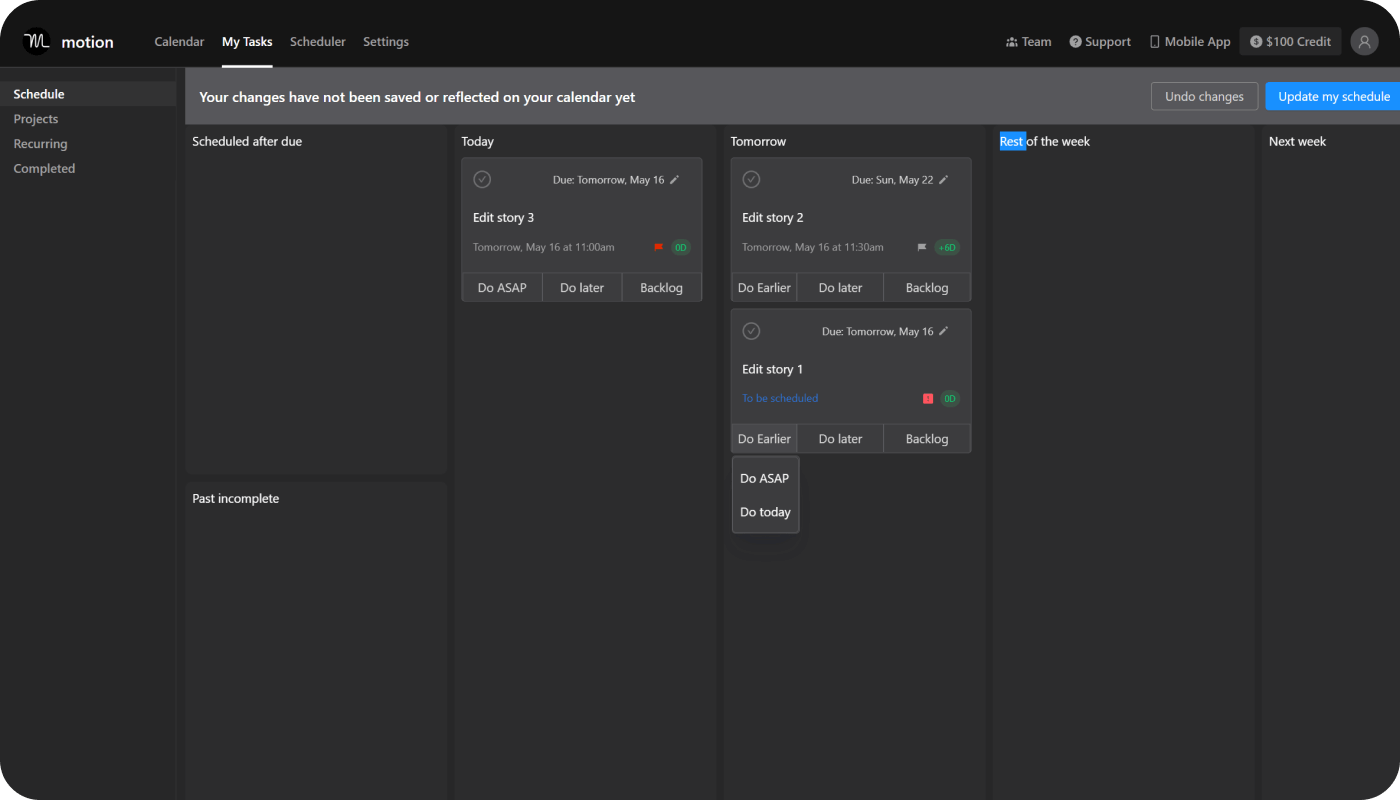
\includegraphics[width=10cm]{img/motion.png}
\caption{Intefaz de calendar}
\end{figure}

\begin{description}
\item[{Motion}] \url{https://www.usemotion.com/calendar}
\end{description}

\pagebreak

\subsection{Generación de tareas}
\label{sec:org1d6eb96}
Asana es el software de gestión de proyectos que te ayuda a planificar
y gestionar de manera más fácil y eficiente el trabajo, una de las
nuevas funciones de Asana es utilizar inteligencia artificial para
poder planificar tareas en base al rendimiento histórico.

Analizar los pasos para cumplir una tarea es una de las partes más
importantes de la planificación y para eso conocer al equipo es
indispensable. 

\begin{figure}[htbp]
\centering
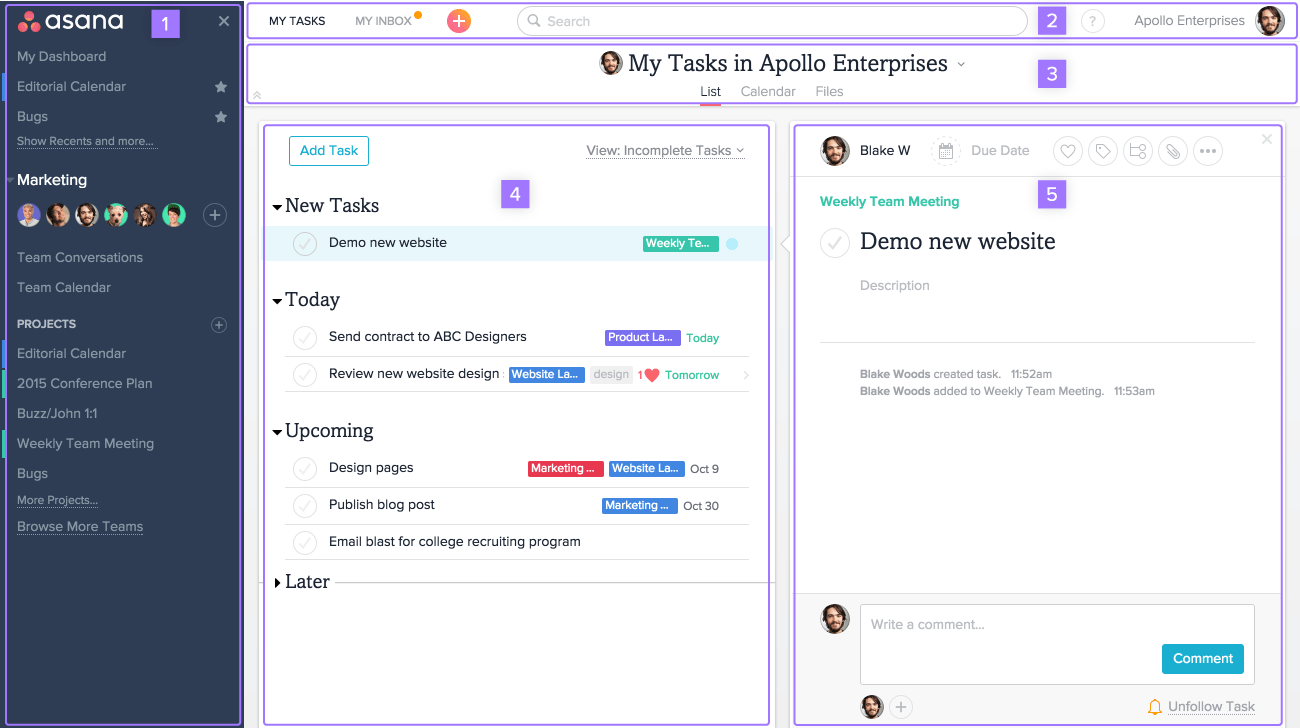
\includegraphics[width=10cm]{img/asana.png}
\caption{Gestor de proyectos de Asana}
\end{figure}

\begin{description}
\item[{Asana AI}] \url{https://asana.com/es/product/ai}
\end{description}

\subsection{Generación de reportes}
\label{sec:org133b763}
Stepsize permite a los encargados de los equipos centralizar todos los
recursos del proyecto y generar reportes sobre el estado del
proyecto.

Reportar el estado del proyecto es una de las principales funciones
del responsable de un proyecto, tener conocimiento a detalle del
trabajo individual de cada uno de los miembros del puede reducir el
tiempo que se invierte en reuniones.

\begin{figure}[htbp]
\centering
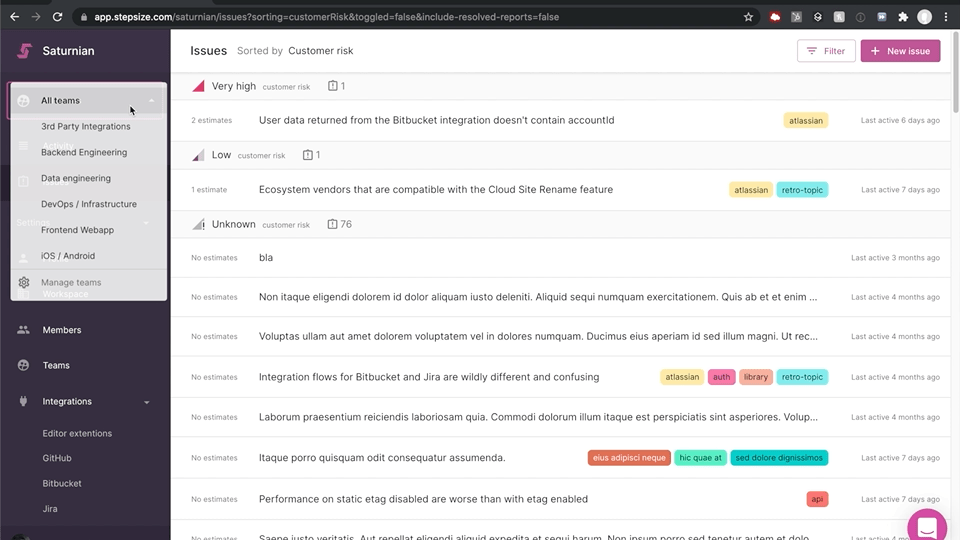
\includegraphics[width=10cm]{img/step-0.png}
\caption{Panel de control de Stepsize}
\end{figure}

\begin{description}
\item[{Stepsize}] \url{https://stepsize.com/}
\end{description}





\section{Conclusión}
\label{sec:org79b2e0e}
A lo largo de esta practica aprendí como las herramientas de
Inteligencia artificial ayudan a las personas a ser mas productivas y
a hacer mas cosas rápidamente, la mayoría de las herramientas que pude
investigar, por lo general, no reemplazan lo que una persona capacitada
puede hacer pero la pueden ayudar a crear mas rápidamente las cosas.
\end{document}